\documentclass[a4paper,conference]{IEEEtran}

\IEEEoverridecommandlockouts
%\usepackage{hyperref}
\usepackage{url}
\usepackage[utf8]{inputenc}
\usepackage[T1]{fontenc}
\usepackage[cmex10]{amsmath}
\usepackage{balance}
\usepackage{subfig}
\usepackage {graphicx}
\usepackage{amssymb}

\title{Improving Predictive Entry of Finnish Text Messages using IRC Logs}


% author names and affiliations
% use a multiple column layout for up to three different
% affiliations
\author{
\IEEEauthorblockA{\ldots\\
\ldots\\
\ldots\\
\ldots}
\and
\IEEEauthorblockA{\ldots\\
\ldots\\
\ldots\\
\ldots}
\and
\IEEEauthorblockA{\ldots\\
\ldots\\
\ldots\\
\ldots}
}



\begin{document}



%\IEEEspecialpapernotice{(Authors' pre-print draft version)}
\maketitle


\begin{abstract}

\end{abstract}

\section{Introduction}
\label{sec:introduction}

\IEEEPARstart{M}{obile} phone text messages are a hugely popular way
of communication, but mobile phones are not especially well suited for
inputting text because of their small size and often limited
keyboard. There are several technological solutions for inputting text
on mobile phones and other limited keyboard devices. This paper is
concerned with a technology called predictive text entry, which utilizes
redundancy in natural language in order to enable efficient text entry
using limited keyboards (typically including 12 keys).

There has been a lot of research into improving predictive text entry
e.g. (...), but research has mainly been concerned with improving the
statistical model, or other technical aspects of the text entry
algorithm. In this paper, we investigate the role of choice of
training data for the accuracy of the text entry system.

There has been work on improving text entry systems by training them
on actual text messages, e.g. (...). Since text messages are difficult
to come by and there are legal restrictions for using them,
open-source text entry systems require alternative sources of training
data, which yield good accuracy. In this paper, we use Internet Relay
Chat (IRC) logs, to train a predictive text input system for Finnish,
and show that this gives significant improvement compared to a
baseline system, which is trained using data from the Finnish
Wikipedia. 

To the best of our knowledge, there have not been earlier inquiries
into using IRC logs for training predictive text entry systems. IRC
log material is nevertheless very well suited for the task, since
there is a lot of material available in different languages. Like text
messages, it resembles spoken language and consists of short messages.

We evaluate our system against the predictive text entry in a number
of widely available mobile phones (...) and show that we get
comparable (better?, only slightly worse?) results. This demonstrates
that it is possible to construct an accurate predictive text entry
system without resorting to actual text message data. Even
optimization of the accuracy of the system can be accomplished without
using actual text message data.

Because Finnish is a morphologically complex language, our system uses
a morphological analyzer for Finnish Omorfi (...). The word forms
found in Omorfi are given probabilities according to their frequency
in the Finnish Wikipedia. These probabilities are combined using
similar probabilitites computed from IRC logs and the final
probability given for a word form is a combination of the probabilities
given by Omorfi and the IRC log model.

Since Omorfi is implemented as a weighted finite-state transducer, we
implemented our predictive text entry system in the weighted
finite-state framework. We used a freely available open-source C++
interface for constructing and utilizing weighted finite-state transducers,
Hfst (...).

This paper is organized as follows: In section \ref{sec:related-work},
we present earlier work in improving the accuracy of predictive text
entry systems. In section \ref{sec:methods}, we explain how to augment
a morphological analyzer with word frequencies computed from IRC logs
and how such a system is used to disambiguate between words
corresponding to an ambiguous input sequence. After this we present
the morphological analyzer, Omorfi, and the Hfst interface in section
\ref{sec:tools} and present the IRC log data used for training out model
and the text message data used for evaluation in \ref{sec:data}. We
evaluate our system in section \ref{sec:evaluation} and present some
general and closing remarks in sections \ref{sec:discussion} and
\ref{sec:conclusions}.

% - Demonstrate the relevance of the research problem.
%   * Predictive text entry works poorly, because it doesn't adequately take 
%     into account the difference between general written language and text 
%     messages.
%   * We need more realistic training data.
%   * Genuine text messages are hard to come by.
% - Instead of text messages, we use IRC logs, which can easily be harvested
%   from the internet (from the public domain?) and which ressemble text 
%   messages.
% - We claim that using IRC Logs and a dictionary we can achieve significant 
%   improvement compared to using only a morphological dictionary
% - We demonstrate that IRC logs can be used to both train and weight a 
%   predictive text entry system for text messages withput resorting to 
%   text message data even for adjusting the weights of component models.
%   (something like that...) 
% - To the best of our knowledge there have been no previous published
%   using IRC logs to train predictive text entry systems.

\section{Related Work}
\label{sec:related-work}

\begin{itemize}
\item Using genre or domain-specific text to train a NLP system is not
  a new idea.The approach has been tested in e.g. automatic
  translation (...) and tagging (...).
\item \cite{Harbusch/2003} Investigate the usefulness of a
  domain-specific lexical model in predictive text entry. They
  established that it is difficult to assemble a good enough purely
  domain-specific lexicon. According to them, the best approach is
  therefore to use a combination of a high coverage general lexicon
  and a domain-specific model, which is exactly what we have done.
\item \cite{Harbusch/2003} are concerned with building systems for very
  specific domains such as school exercises ad scientific texts. They
  do not really address the question of what would constitute
  practical training material for a general text message system. We
  are expressly interested in improving text entry using widely
  available materials.
\end{itemize}

\section{The Task of Predictive Text Entry}

The keypad of a typical mobile phone has twelve keys for typing
numbers and symbols. Additionally there are function keys, which are
used for various other purposes. The typical layout uses ten keys for
typing numbers and letters and the remaining two keys for typing
special symbols, e.g. "*", "\#", "+" and <SPACE>. Figure
\ref{fig:keypad} shows a typical layout for a mobile phone keyboard.

The letters of the English alphabet are distributed between the keys
from 2 to 9, in such a way that each key can be used to type three or
four letters.

For most languages whose alphabet differs from the English alphabet,
number keys are also used to input the remaining symbols, which are
not found in the English alphabet. E.g. the three Finnish letters not
found in the English alphabet "å'', "\"{a}" and "\"{o}" are typed
using key 2 in case of "å" and "\"{a}" and key 6 in case of "\"{o}".

Since each key from 2 to 9 corresponds to at least three different
letters, every sequence of numbers encodes many different letter
sequences. The letter sequences are called suggestions. Predictive
text entry is the task of finding the correct suggestion corresponding
to the number sequence received as input from a user of the mobile
phone. The correct suggestion is the letter sequence the user
intended, typically a word.

Our method is based on lexical models derived from different
sources. In this paper we consider only the problem of disambiguating
between suggestions, which are known to the lexical models. Thus we do
not consider the problem of finding the correct suggestion for number
sequences which cannot correspond to any of the words known to the
lexical models. Neither do we consider the problem of finding the
correct suggestion based on partial input.

\begin{figure}
\begin{center}
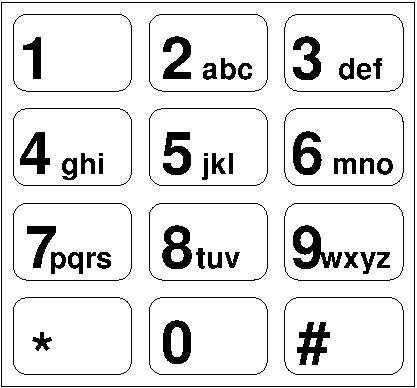
\includegraphics[width=1.5in]{keypad.pdf}
\end{center}
\caption{The layout of a typical twelve-key mobile phone keyboard.}
\label{fig:keypad}
\end{figure}

\section{Combining a Morphological Lexicon and IRC Logs}
\label{sec:methods}

Our goal is to first combine two probabilistic lexicons, to build a
probabilistic model which (i) has broad lexical coverage and (ii)
gives a good approximation of the probabilities of word forms in text
messages. We then transform the model so that it can be used as a
machine, that takes number sequences such as "2452" as input. It
outputs the list of Finnish words that can correspond to the input,
when typed on a cell phone. The output contains only those words,
which are known to the lexicons. The words are appended with a
probability, which is computed from the probabilities given by the
lexicons used to construct the model.

One of the lexicons we use is derived from the Finnish open-source
morphological analyzer Omorfi. The other lexicon we construct from a
corpus of IRC logs.

We have chosen to implement our system using weighted finite-state
machines, partly because the morphological analyzer Omorfi is
implemented as a WFST, but also because they provide a flexible way of
combining models to build language technology applications.

\subsection{Weighted Finite-State Transducers}

%The weighted language model in our finite-state language model is based
%on morphological dictionary of the language created in traditional
%finite-state morphology framework\cite{beesley/2003}. The weights in
%this system will be basic scaled unigram weights transformed in
%finite-state form by $w = -\log \frac{f}{cs}$ where $w$ is the weight,
%$f$ is the frequency of token and $cs$ the size of corpus in
%tokens. For tokens that do not exist maximum weight of $w_{max} =
%-\log \frac{1}{cs+1}$ is used.  The probabilities are gained by
%extracting the word frequencies from a large scale corpus such as
%wikipedia~\cite{pirinen/2010/lrec}. The basic unigram weighting system
%can be fine-tuned, especially on part of unknown words, by composing
%additional weights based on e.g. morphological complexity, as
%suggested in \cite{karlsson/1992}, which can be easily modeled in
%weighted finite-state form as suggested e.g. in\cite{schiller/2005}

Finite-state transducers are a class of computational models, which
rewrite input strings to output strings \cite{beesley/2003}. The input
string $s_i$ and its output string $s_o$ are called a correspondence
and written $s_i\mathrm{:}s_o$. If $T$ is a transducer, we write
$s_i\mathrm{:}s_o \in T$, iff $T$ rewrites $s_i$ as $s_o$, i.e. accepts the correspondence $s_i\mathrm{:}s_o$.

Classical examples of language technological applications
implemented as finite-state transducers, are morphological analyzers,
which rewrite an input word e.g. "dog" into a set of morphological
analyses $\{$"dog+NOUN+SG", "dog+VERB+INF"$\}$. Here "dog" is the
input string in two correspondences.

Our system is implemented using weighted finite-state transducers
(WFSTs). These are an extension of finite-state transducers, where
every correspondence $s_i\mathrm{:}s_o$ between an input string $s_i$
and an output string $s_o$ receives a weight $\mathrm{w}_T(s_i\mathrm{:}s_o)$,
where $T$is the transducer. The weight is a floating point number. 

The weights in our system represent probabilities, which have been
transformed into so called penalty weights using the map $p \mapsto
-\log p$ in order to avoid underflow in computer arithmetics. Since
probability $0$ corresponds to an infinite penalty weight, we say that
a transducer $T$ gives infinite weight to correspondences it doesn't
accept. Weight arithmetics is performed in the tropical semiring, so
addition of weights $w_1 \oplus w_2$ corresponds to taking their
minimum $\min(\{w_1,w_2\})$ and multiplication $w_1 \otimes w_2$
corresponds to ordinary addition of floating point numbers $w_1 + w_2$.

Akin to ordinary transducers, WFSTs can be combined using
different binary algebraic operations or modified using unary
algebraic operations to yield new WFSTs. Our system uses two unary and three binary operations:
\begin{itemize}
\item {\bf Projection $\mathrm{P}(T)$:} A unary operation, whose result
  rewrites a string $s_i$ into itself, iff the argument rewrites $s_i$
  into any output string $s_o$. The weight given to each correspondence
  $s_i:s_i$ is
  \begin{equation}
    \bigoplus_{s_i\mathrm{:}s_o \in T} \mathrm{w}_T(s_i\mathrm{:}s_o)
  \end{equation}
\item {\bf scaling $\mathrm{W}_k(T)$,where $k \in \mathbb{R}$:} A unary operation, whose result accepts the same correspondences $s_i\mathrm{:}s_o$ as $T$ with weight $k\cdot \mathrm{w}_T(s_i\mathrm{:}s_o)$. Here we use regular multiplication of floating point numbers (not $\otimes$).
\item {\bf Disjunction $S \cup T$:} (sometimes called union) A binary
  operation, whose result rewrites an input strings $s_i$ into the
  output string $s_o$, iff one of the argument transducers writes
  $s_i$ to $s_o$. The weight given each correspondence
  $s_i\mathrm{:}s_o$ is
  \begin{equation}
    \mathrm{w}_S(s_i\mathrm{:}s_o) \oplus \mathrm{w}_T(s_i\mathrm{:}s_o)
  \end{equation}
\item {\bf composition $S \circ T$:} A binary operation, whose result
  writes an input string $s_i$ into an output string $s_o$, iff the
  first argument rewrites $s_i$ as some string $t$ and the second
  argument rewrites $t$ to $s_o$. The weight given each correspondence
  $s_i\mathrm{:}s_o$ is
  \begin{equation}
    \bigoplus_{s_i\mathrm{:}t \in S, t\mathrm{:}s_o \in T} \mathrm{w}_S(s_i\mathrm{:}t) \otimes \mathrm{w}_T(t\mathrm{:}s_o)
    \end{equation}
\item {\bf Subtraction $S - T$:} A binary operation whose result accepts those correspondences in $S$, which are not accepted by $T$. The weight remains the same, so
  \begin{equation}
    \mathrm{w}_{S-T}(s_i\mathrm{:}s_o) < \infty \Rightarrow \mathrm{w}_{S-T}(s_i\mathrm{:}s_o) = \mathrm{w}_{S}(s_i\mathrm{:}s_o)
  \end{equation}
\end{itemize}
For a more thorough discussion on WFSTs, see \cite{openfst/2007}.

\subsection{Component of the predictive text entry system}

Our system is constructed from three WFSTs, which are combined using
disjunction and composition:

\begin{itemize}
\item A transducer $[\mathrm{Num}\rightarrow\mathrm{Text}]$, which
  rewrites number sequences as letter sequences mimicing the way the
  keypad of a 12-key cell phone
  works. E.g. $[\mathrm{Num}\rightarrow\mathrm{Text}]$ would rewrite
  $23$ as the strings "ad", "ae", "af", "bd", "be", "bf", "cd", "ce"
  and "cf". Each correspondence in $[\mathrm{Num}\rightarrow\mathrm{Text}]$
  receives equal weight.
\item A lexicon transducer $L_O$, which rewrites word forms as them
  selves (i.e. gives an identity correspondence) and associates a
  penalty weight corresponding to a probability to known word
  forms. The probability is based on corpus frequencies. An English
  lexicon might e.g. accept the correspondence "be":"be" with penalty
  weight $5.41$ corresponding to the probability $0.39\%$.
\item A domain specific lexicon transducer $L_I$, which also
  associates penalty weights to word forms, but the probabilities have
  been computed from some source which resembles the language used in
  text messages (in our case IRC logs).
\end{itemize}

The lexicon transducer $L_O$ is derived from an existing morphology $M$
(in this paper we use the open-source finite-state morphology for
Finnish Omorfi). The morphological analyzer is converted to a lexicon
using projection, which throws away the morphological analyses and
leaves a transducer which accepts wordforms. Hence 
\begin{equation}L_O = \mathrm{P}(M)\text{.}\end{equation}

Schematically our system works by looking up a number sequence in
$[\mathrm{Num}\rightarrow\mathrm{Text}]$ to find all possible letter
strings associated to the sequence and then performing a lexicon
lookup in both of the lexicons $L_O$ and $L_I$ to see which of the
letter sequences are actually words. Each of the words receives some
(possibly infinite) weight from both $L_O$ and $L_I$. In case, either
one of the lexicons gives an infinite weight, it will be replaced by
some large penalty $w_{max}$. For each candidate word, a weighted
average is computed from these penalties and this is the total penalty
weight of the candidate word. Predictive text entry will offer the
candidates in order of increasing penalty weight.

In practice this approach is not feasible, because
$[\mathrm{Num}\rightarrow\mathrm{Text}]$ will over-generate hugely
(e.g. for a string of ten numbers at least $3^{10} = 59049$ letter
sequences are generated and need to be looked up in the
lexicons). This is why we compile all three transducers into one
transducer using composition, disjunction and subtraction. The
transducer performs translation into letter sequences and lexicon
lookup simultaneously thus avoiding over-generation.

\subsection{Combining the Component Lexicons}

In this subsection we explain, how the lexicons $L_O$ and $L_I$ are
combined with the transducer $[\mathrm{Num}\rightarrow\mathrm{Text}]$
to form the transducer which performs predictive text entry. We first
derive a formally correct way to combine the transducers and then show
how it can be done simpler, without sacrificing accuracy.

As we explained above, it may happen that some word forms are found in
one lexicon but not the other. In that case we want to replace the
infinite weight given by one of the lexicons by a large penalty weight
$w_{max}$, which is greater than the weight given by the lexicons for
any accepted word form. Therefore we disjunct the lexicons with the
language $U_{max}$, which accepts all words and gives them weight
$w_{max}$. For the lexicon $L_O$, the result $L_O \cup U_{max}$ will
accept any word form $s$ and give it weight
$\mathrm{w}_{L_O}(s\mathrm{:}s)$, if it is accepted by $L_O$ and
$\mathrm{w}_{max}$ otherwise. The same applies for $L_I \cup U_{max}$.

We want to construct such a transducer $L$, that $\mathrm{w}_L(s\mathrm{:}s)$
is a weighted average of the weights $\mathrm{w}_{L_I \cup U_{max}}(s\mathrm{:}s)$ and
$\mathrm{w}_{L_O \cup U_{max}}(s\mathrm{:}s)$, i.e.
\begin{equation}
  \mathrm{w}_L(s\mathrm{:}s) = k\cdot \mathrm{w}_{L_I}(s\mathrm{:}s) + (1 - k)\cdot \mathrm{w}_{L_O}(s\mathrm{:}s)\text{, where }0\leq k \leq 1\text{.}
\end{equation}
Notice that we use regular addition and multiplication of floating
point numbers. We can easily represent the transducer using scaling, disjunction and composition
\begin{equation}
  L = \mathrm{W}_k(L_I \cup U_{max}) \circ \mathrm{W}_{1-k}(L_O \cup U_{max})
\end{equation}

There is a problem with the language $L$. It will accept every
string of letters, which is a performance concern, as we explained
above. Therefore we need to subtract the language of all strings that
are not in $L_I$ or $L_O$. Hence the final lexicon is
\begin{equation}L_{I\vee O} = L - (U - (L_I \cup L_O))\text{,}\end{equation}
where $U$ is the language of all letter strings.

Finally we can compose $[\mathrm{Num}\rightarrow\mathrm{Text}]$ with
$L_{I\vee O}$ in order to get a transducer, which transforms number
sequences to word forms.

In the construction of the composite lexicon $L$, we used the floating
point constant $k$. This constant needs to be estimated
experimentally. In section \ref{sec:evaluation}, we show that the
constant can be estimated without resorting to a corpus of text messages.

The method which we described is fairly contrived, so we wanted to try
out a simplifyed way to combine the lexicons
\begin{equation}
  L_{I\vee O}' = \mathrm{W}_k(L_I) \cup \mathrm{W}_{1-k}(L_O)\text{, where }0 \leq k \leq 1\text{.}
\end{equation} 
The weight given to a word form $s$ by $L_{I\vee O}'$ is not a linear
combination of the scaled weights given by $L_I$ and $L_O$. Instead
it's the minimum of the scaled weights
$\mathrm{w}_{L_I}(s\mathrm{:}s)$ and $\mathrm{w}_{L_O}(s\mathrm{:}s)$.
Tests showed negligible difference in accuracy between the methods,
which lead us to use the simplifyed method in practice.

\subsection{Using a Combination of Lexicons for Predictive Text Entry}

The lexicon $L_{I\vee O}'$ is used by performing lookup for number
sequences. The result is a finite set of word forms with weights. The
system gives suggestion in order of weight.

Using the Hfst interface, we can convert the transducer into a fast
lookup format \cite{conf/fsmnlp/Silfverberg2009}, whose throughput is
about $100000$ number sequences per second, which is more than
sufficient for predictive text entry.

\section{Tools and Resources}
\label{sec:tools}

To implement the full system we have used only freely available open source
tools and resources that anyone can download from the Internet to reproduce the
results. For the finite-state system we have selected the HFST
tools\footnote{\url{http://hfst.sf.net}}, which is relatively complete
reproduction of the classical tools of finite-state
morphology\cite{beesley/2003}. Similarly we have downloaded a freely available
Finnish finite-state morphological analyser
omorfi\footnote{\url{http://home.gna.org/omorfi/}} for our language model
data\cite{pirinen/2011/nodalida}. For further training of the language model we
have used the Finnish
Wikipedia\footnote{\url{http://dumps.wikimedia.org/fiwiki/latest/}} as corpus
to acquire the unigram probabilities\cite{pirinen/2010/lrec}.

\subsection{Tools}

In our setup we use unmodified version of HFST tools for creation, manipulation
and use of finite state transducers\cite{hfst/2011}. This means that we have
not needed to prepare any specialised algorithms for application of the t9
predictive input model. This basically means that it can be used on any of
current or future finite-state systems as long as they implement needed subset
of finite-state algebra as defined in \ref{sec:methods}.

For processing of corpora we have used standard GNU tools like coreutils as
well as bash and python scripting languages. The source code of the full system
used for building, applying and evaluation of the full system is available
under free
licence\footnote{\url{http://hfst.svn.sourceforge.net/viewvc/hfst/trunk/cla-2011-article/}}.

\subsection{Data}
\label{sec:data}

For language model we have selected to use ready-made free open source
finite-state implementation of Finnish language\cite{pirinen/2011/nodalida}.
The language model here is meant for parsing running text consisting mainly of
standard written Finnish language, which is relatively far from the language
sms text messages.  To train the language model we have used
the Finnish Wikipedia data to add unigram probabilities to word forms that are
recognised by the language model we are using. 

\subsubsection{IRC Logs}
IRC (Internet Relay Chat) VIITE? is a real-time messaging network. It is mainly used for group communication, but also enables private one-on-one discussions. The group communication happens on channels, similar to chat rooms, of which some are private and require a password to enter. The IRC logs we use are from a public channel directed mainly to the members of a local student organization. The topic of the discussion varies a lot making the log quite versatile as test and teaching material.

IRC discussions tend to be rather informal, and thus the language used is casual, resembling the spoken language, as is also the case with text messages. In Finnish this  means e.g. shortening words from the end and using different word forms than formal written language does.

The IRC logs used in this research contain 385303 words after omitting everything that does not consist of letters, an apostrophe (') and a hyphen (-); the three elements that are used to form Finnish words.

\subsubsection{Text Messages}

Authentic text messages were collected for testing purposes via requests in the social media from 12 volunteers, aged between 20 and 35. The messages contain 10851 words after the same trimming that was performed to the IRC logs.

\section{Evaluation}
\label{sec:evaluation}

Our goal was to test whether adding some understanding of spoken language to the lexicon of a predictive text model improves its quality. We also aimed to find out how suitable IRC logs are for this purpose. We used a morphological analyser for Finnish as a baseline model. Our hypothesis is that the language in IRC logs, being often of casual nature, resembles the language used in text messages and can therefore be used as a source for creating models that understand spoken language.


\subsection{Creating the models and determining penalty weights}
\label{sec:weighting}
To create a model with and understanding of spoken language, we started out by separating one tenth of the IRC logs and setting it aside for testing purposes, and used the rest of the logs to build the model. We counted the frequencies of the words and built a transducer of them, containing weights based on the frequencies. PAINOJEN LASKUKAAVA? The weights were processed (…) to the form of penalty weights, where small values mean high desirability.

After creating the model for spoken language, we combined it with the baseline model, i.e. the morphological analyser. We scaled the weights of the baseline model and the spoken language model to fit the same scale by MIIKKA KERTOO JOTAIN? and tried out different ways of prioritising the spoken language compared to the literal language contained by the baseline model. We created 11 combination models, giving the spoken language a propositional weight scaling from 0.0 (no penalty weight) to 1.0 (maximum penalty weight) with an interval of 0.1. 

Both the baseline model and the combination model understanding spoken language take number sequences as an input and return an analysis of which words would match that sequence, sorted according to the penalty weights of the words. In cases where a word is recognised by both models, the one with a smaller penalty weight (i.e. better rating) will be chosen.

We tested the combination model with the one tenth of the IRC log set aside for testing. 94.37 \% of the words were successfully analysed. Of all the weighted combination models, the one with the weight 0.2 for the spoken language model and the 0.8 weight for the baseline model recognised the most words on the first try (see MIIKAN KUVA).

\subsection{Assessing the difficulty of the test material}
\label{sec:difficulty}
To ensure the test results were not merely a result of coincidentally having chosen an exceptionally easy tenth of the IRC logs, we ran the same tests for each of the other tenths as well, creating the combination models using the rest of the logs, using the optimal weighting (see \ref{sec:weighting}). The amount of the words recognised was between 93.95 and 94.99 \% in each case, with an average of 94.51 \%. This means that the original tenth of the logs used for testing is quite similar to the other tenths in terms of difficulty for the model, and we have no reason to assume the choice of the test material would significantly bias the results.

\subsection{Testing with text messages}
 
We then used the text message data for testing. 91.07 \% of the words were analysed correctly. The text message data also received the best results with the weighting 0.2 for the spoken language model and 0.8 for the baseline model, with which 75.16 \% of the words were recognised on the first attempt.

We also ran tests with the text message data on the alternative combination models created for testing the difficulty of the original combination model (see \ref{sec:difficulty}). The amount of successfully analysed words range between 91.06 \% and 91.18\%, and from 75.02 \% to 75.42 \% of the words were recognised at the first attempt. 

The results for correct first guesses have an average of 75.22 \%, with a standard deviation of 0.10 percentage points. If the results follow the normal distribution, 99.7 \% of them should be within 3 standard deviations from the average, i.e. between 74.92 \% and 75.52 \%. We do not know whether the results are normally distributed, but this gives us a rough idea of what the results are expected to look like.

% omorfi, tekstarit
\begin{table}
\begin{center}
\begin{tabular} {l c r}
 & Baseline & Combination \\
 \hline
Recognised on first try \rule{0pt}{2.6ex} & 55.10 \% & 75.12 \% \\
Recognised in 3 tries & 72.18 \% & 85.81 \% \\
Recognised & 81.37 \% & 91.07 \% \\
\hline
 & & \\
\end{tabular}
\end{center}
\caption{Recall for the baseline system (using only the morphological analyzer Omorfi) and our system using the weight coefficient 0.2 for the IRC log model and 0.8 for the morphological analyzer.}
\label{tab:recall}
\end{table}


To confirm our assumption that adding the understanding of spoken language indeed improves the quality of the results, we ran the text message test data through the baseline model to see how much the spoken language model affects the results. The difference between the results achieved with the baseline and the combined model is noticeable. The baseline gave a correct analysis for 81.37 \% of the words. Only 55.10 \% of the words were given the correct analysis at the first attempt.

\begin{table}
\begin{center}
\begin{tabular} {l c c}
System & Recall 1st guess & Recall 1st to 3rd guess\\
\hline
Nokia 2600 \rule{0pt}{2.6ex}  & 74.19\%          & 83.68\%\\
Nokia C7     & 70.97\%          & 83.87\%\\
Samsung SGH-M310 & 74.19\%      & 83.68\%\\
Our system & 64.52\% & 80.65\%  \\
\hline
\end{tabular}
\end{center}
\caption{Recall fot the predictive text entry of three different mobile phones and our system using 31 words chosen at random from the text message test material.}
\end{table}

To determine the significance of the differences between the results from the baseline model and the combination model, we ran a Wilcoxon paired rank test which is suitable for data that cannot be guaranteed to follow the normal distribution. We compared the percentages of correct first attempts with the baseline model and the ten different combination models. Since the test requires equally big sets of test data, we used the baseline model result as a counterpart for each of the different combination model results. The test gave a p-value of 6.34e-05, which means that we can quite confidently say the results differ quite clearly.



\begin{figure*}[!t]
\centerline{\subfloat[The first guess is correct.]{\includegraphics[width=3.5in]
  {accuracy_first_guess.pdf}}
\hfil
\subfloat[Correct guess found among the three first guesses.]{\includegraphics[width=3.5in]
  {accuracy_first_to_third_guess.pdf}}}
\caption{The recall of our algorithm using different linear combinations of the weights given by the morphological analyzer and the IRC log transducer. On the x-axis we give the relative weight of the IRC log transducer and on the y-axis we give the recall. The dotted line gives the recall for the IRC log test material and the solid line gives the recall for the text message test material. Peak recall for the text message test material is 75.8\% for the first guess and 86.5\% for the three first guesses.}
\label{fig:AccuraciesIRCMaterial}
\end{figure*}

\begin{figure}[!t]
\begin{center}
\includegraphics[width=3.5in]{accuracy_as_function_of_data_size.pdf}
\end{center}
\caption{Recall for the first guess as a function of the number of words in the training data. The increase in recall clearly levels out as we use more training data. The increase in recall when going from $200000$ words of training data to $350000$ words of training data is only about 1.3 percentage points.}
\label{fig:SaturationGraph}
\end{figure}

\section{Discussion and Future Work}
\label{sec:discussion}

This work demonstrates that using simple methods we can improve a lot.\ldots

In this paper we used readily available language model geared towards parsing
running texts of literary written Finnish. It would be interesting to see if
modifying the language model towards the standard spoken Finnish dialect
might yield a significant increase in recall.

The demonstrated model only considers unigrams for probability
likelihood maximisation. It has been demonstrated that it is possible
to extend these models trivially to arbitrary n-gram and varigram
models \cite{Silfverberg/2011}, and this should be explored to see if
there's improvement for wider statistical models in task of predictive
text input for mobile text messages.

Finally we have only performed our experiment for Finnish, but we believe that
same methods will apply to at least most of the latin abjad based languages
with no modifications excepting the orthographic conventions---such as accent
dropping---on some texting cultures.

\section{Conclusion}
\label{sec:conclusions}

\ldots \balance
\section*{Acknowledgment}
Lorem ipsum dolor sit amet, consectetur adipisicing elit, sed do eiusmod tempor incididunt ut labore et dolore magna aliqua. Ut enim ad minim veniam, quis nostrud exercitation ullamco laboris nisi ut aliquip ex ea commodo consequat.

% We the people thank the HFST research team and the staff of University of
% Helsinki for fruity discussions as well as the anonymous reviewers for
% good suggestions.
\
\bibliographystyle{IEEEtran}
\bibliography{cla2011}




% that's all folks
\end{document}


